% !TEX encoding = IsoLatin2  % notwendige Zeile für Mac-Benutzer (muss als Kommentar stehen); Windows-Benutzer können die Zeile löschen.

% LaTeX-Vorlage Version 3.1,  Juli 2011
% erstellt von Dr. Andreas Drauschke (andreas.drauschke@technikum-wien.at) und Dr. Susanne Teschl (susanne.teschl@technikum-wien.at)
% geringfügig adaptiert von Harald Stockinger (harald.stockinger@technikum-wien.at)

 
\documentclass[a4paper,bibtotoc,oneside]{scrbook} 
% Für kurze Arbeiten wäre auch die Dokumentklasse "scrartcl" ausreichend. In diesem Fall ist "section" die höchste Ebene ("chapter" gibt es dann nicht).
% \documentclass[a4paper,bibtotoc,oneside]{scrartcl}

%\usepackage{cclicenses}

% javascript highlightning support
\usepackage{listings}
\usepackage{color}
\definecolor{lightgray}{rgb}{.9,.9,.9}
\definecolor{darkgray}{rgb}{.4,.4,.4}
\definecolor{purple}{rgb}{0.65, 0.12, 0.82}

\lstdefinelanguage{JavaScript}{
  keywords={typeof, new, true, false, catch, function, return, null, catch, switch, var, if, in, while, do, else, case, break},
  keywordstyle=\color{blue}\bfseries,
  ndkeywords={class, export, boolean, throw, implements, import, this},
  ndkeywordstyle=\color{darkgray}\bfseries,
  identifierstyle=\color{black},
  sensitive=false,
  comment=[l]{//},
  morecomment=[s]{/*}{*/},
  commentstyle=\color{purple}\ttfamily,
  stringstyle=\color{red}\ttfamily,
  morestring=[b]',
  morestring=[b]"
}
\lstset{
   language=JavaScript,
   backgroundcolor=\color{lightgray},
   extendedchars=true,
   basicstyle=\footnotesize\ttfamily,
   showstringspaces=false,
   showspaces=false,
   numbers=left,
   numberstyle=\footnotesize,
   numbersep=9pt,
   tabsize=2,
   breaklines=true,
   showtabs=false,
   captionpos=b
}

% verlinkte Querverweise im pdf
\usepackage{hyperref}

% deutsche Anpassungen
\usepackage[utf8]{inputenc}
\usepackage[T1]{fontenc}
\usepackage[ngerman]{babel}


% mathematische Symbole
\usepackage{amsmath,amssymb,amsfonts,amstext}

% Kopfzeilen frei gestaltbar
\usepackage{fancyhdr}
\lfoot[\fancyplain{}{}]{\fancyplain{}{}}
\rfoot[\fancyplain{}{}]{\fancyplain{}{}}
\cfoot[\fancyplain{}{\footnotesize\thepage}]{\fancyplain{}{\footnotesize\thepage}}
\lhead[\fancyplain{}{\footnotesize\nouppercase\leftmark}]{\fancyplain{}{}}
\chead{}
\rhead[\fancyplain{}{}]{\fancyplain{}{\footnotesize\nouppercase\sc\leftmark}} 

% Farben im Dokument möglich
\usepackage{color}

% Schriftart Helvetica
\usepackage{helvet}
\renewcommand{\familydefault}{cmss} 

% Graphiken einbinden: hier für pdflatex
\usepackage[pdftex]{graphicx}

\usepackage{array}

% Höhe und Breite des Textkörpers etwas grösser definieren
\setlength{\textheight}{225mm}
\setlength{\textwidth}{1.05\textwidth}

% weniger Warnungen wegen überfüllter Boxen
\tolerance = 9999
\sloppy

% Anpassung einiger überschriften 
\renewcommand\figurename{Abbildung}
\renewcommand\tablename{Tabelle}

\begin{document}

% Kopf- und Fusszeilen initiieren
\pagestyle{fancy}
\pagenumbering{Alph}

% Deckblatt:
\thispagestyle{empty}
\begin{picture}(0,0)
\color{white}\sffamily
\put(-101,-749){
\includegraphics[width=1.002\paperwidth, height=\paperheight]{BM_2011.pdf}}
\put(220,-670){
\includegraphics[width=0.5\textwidth]{FHTW_Logo_4c.pdf}}
\put(-30, -20){\bfseries\huge BACHELORARBEIT}
% Titel des Studienganges einfügen:
\put(-30,-50){\Large im Studiengang Bachelor Informatik}
% Titel der Arbeit einfügen:
% Die Minipage wird gesetzt, damit auch mehrzeilige Titel möglich werden.
\put(-32,-150){
\begin{minipage}{14cm}
\bfseries\huge Software-Test von Web-Applikationen
\end{minipage}
}
% Name der Autorin/des Autors eingeben:
\put(-30,-250){\large Ausgeführt von: Bernhard Posselt}
% Personenkennzeichen der Autorin/des Autors eingeben:
\put(-30,-270){\large Personenkennzeichen: 1010257029}
% Name der Begutachterin/des Begutachters eingeben:
\put(-30,-310){\large Begutachter: Benedikt Salzbrunn, MSc}
\put(-30,-350){\large Wien, \today} % das Datum des letzten Kompilierens wird automatisch eingesetzt
\color{black}
\end{picture}

\newpage


\section*{Eidesstattliche Erklärung}\thispagestyle{empty}
\glqq Ich erkläre hiermit an Eides statt, dass ich die vorliegende Arbeit selbständig angefertigt habe. 
Die aus fremden Quellen direkt oder indirekt übernommenen Gedanken sind als solche kenntlich gemacht. 
Die Arbeit wurde bisher weder in gleicher noch in ähnlicher Form einer anderen Prüfungsbehörde vorgelegt
und auch noch nicht veröffentlicht. Ich versichere, dass die abgegebene Version jener im Uploadtool entspricht.\grqq\\[5\baselineskip]
\rule{5cm}{0.2pt}\hfill\rule{5cm}{0.2pt}\\
\phantom{Datum }Ort, Datum\hfill Unterschrift\hspace{15mm}

\newpage


\section*{Kurzfassung}\thispagestyle{empty}
Die Durchführung und Erstellung von automatisierten Tests für Web-Applikationen unterscheidet sich von klassischen Applikationen: Aufgrund der komplexeren Infrastruktur und Modularisierung werden zusätzliche Testfälle und Strategien benötigt um Web-Applikationen ausreichend abzudecken und eine fortwährende Qualität zu gewährleisten. Diese Arbeit soll Möglichkeiten für den Test von Web-Applikationen anhand eines Projektes aufzeigen und Anpassungen und Anwendung der vier Testformen des V-Modells: Unit Test, Integration Test, System Test und Acceptance Test. 

\vfill
\paragraph*{Schlagwörter:} Softwaretest, Web

\newpage

\section*{Abstract}\thispagestyle{empty}
Creation and execution of automatic web application tests is different from tests of classic applications. A more complex infrastructure and modularisation require additional testcases and strategies to guarantee a good enough test coverage which in return ensures constant quality. This thesis highlights various possibilities to test web applications based on a real world project and shows how to use and adjust the V-Model's four test methods: Unit Test, Integration Test, System Test and Acceptance Test.

\vfill
\paragraph*{Keywords:} web applications, automatic tests, webtest
\newpage

%\section*{Danksagung}
%\thispagestyle{empty}
%Text Text Text Text Text Text Text Text Text Text Text Text Text Text Text Text
%\newpage

\tableofcontents\thispagestyle{empty}
\newpage

\pagenumbering{arabic}
\setcounter{page}{1}

% Falls die Kapitelüberschriften zu lang für die Kopfzeile oder das Inhaltsverzeichnis sind, so erzielt man
% dort Kurzformen der Kapitelbezeichnungen mittels:
% \chapter[Kurzform]{Lange überschrift}
\chapter{Einführung}
Immer mehr unserer Alltagsgeräte ermöglichen einen Zugang zum Internet. Besonders der Markt für mobile elektronische Geräte hat in den letzten Jahren ein rasantes Wachstum erlebt: Im Jahr 2011 wurden erstmals mehr mobile Geräte verkauft als PCs (Abbildung \ref{Abb1}).

Aufgrund des starken Wachstums dehnt sich der Markt für Software-Applikationen auch auf mobile Geräte aus, welche zum Großteil andere Betriebssysteme und Applikations-Frameworks verwenden als traditionelle Computer (Abbildung \ref{Abb2}). Viele dieser Plattformen erfordern das Erlernen von unterschiedlichen Programmiersprachen, Frameworks und Betriebssystemen \cite{android}\cite{ios}. Will ein/eine Software-EntwicklerIn eine Applikation plattformübergreifend anbieten, erfordert dies daher einen höheren Zeit- und Kostenaufwand.

\begin{figure}[h!]
\centering
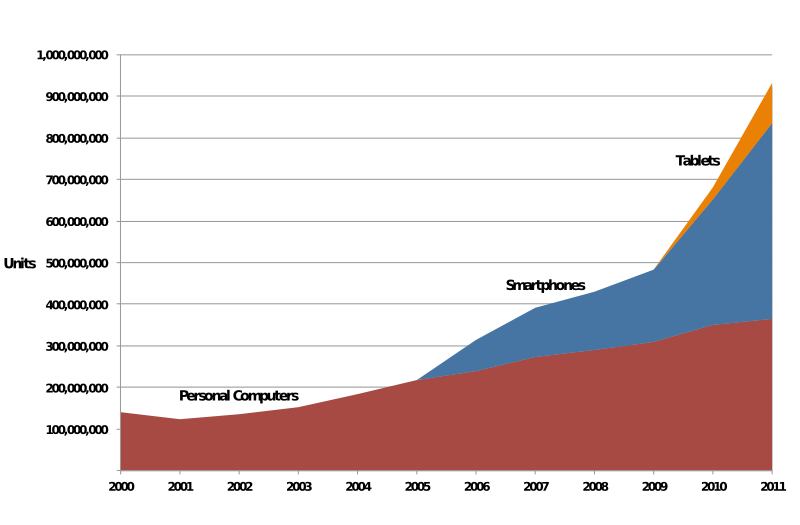
\includegraphics[width=150mm]{img/globaldevicesales.png}
\caption[Entwicklung der PC und Mobilgerätverkäufe]{Entwicklung der PC und Mobilgerätverkäufe \cite{devicesales}[S. 6]}\label{Abb1}
\end{figure}
% TODO: grafik verbessern, klarer machen

Dieses Problem der Fragmentierung und des damit verbundenen immer höheren Portierungsaufwandes kann mit einer Web-Applikation gelöst werden. Soll sich diese auch noch gut in das jeweilige System integerieren, können Frameworks wie z.B. PhoneGap \cite{phonegap} verwendet werden. Diese Frameworks bieten über JavaScript einen Zugriff auf native Funktionen der mobilen Betriebssysteme, womit der Portierungsaufwand deutlich reduziert werden kann. 

\begin{figure}[h!]
\centering
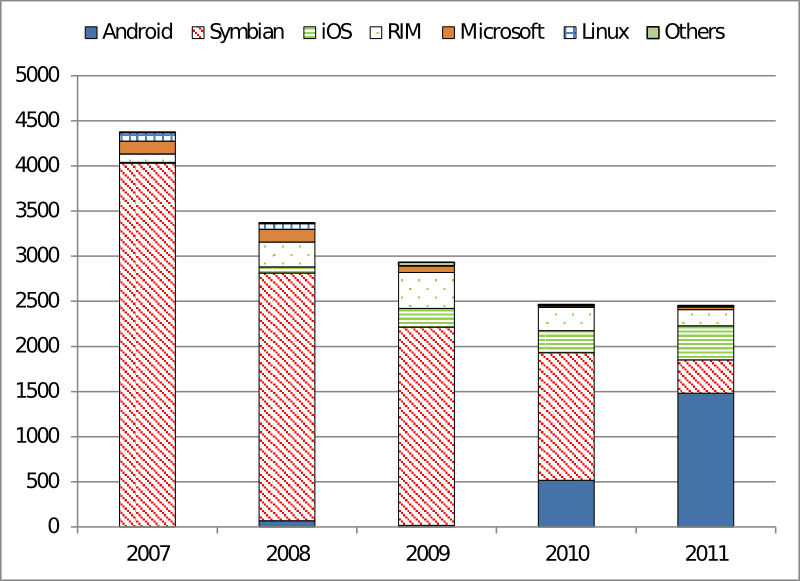
\includegraphics[width=130mm]{img/operatingsystems.png}
\caption[Marktanteil mobiler Betriebssysteme]{Marktanteil mobiler Betriebssysteme \cite{smartphone}[S. 22]}\label{Abb2}
\end{figure}

\section{Problemstellung}
Aufgrund der Vielfalt an unterschiedlichen Web-Browsern erhöht sich jedoch auch der Testaufwand der Applikation. Die Browser implementieren die vom W3C vorgeschlagenen Standards ab und zu anders und in unterschiedlicher Geschwindigkeit. Nicht selten kommt es vor, dass gewisse Funktionen nur in einer eingeschränkten Auswahl von Web-Browsern voll funktionsfähig sind und zusätzliche Anpassungen erfordern. \cite{caniuse}

Ein weiteres Problem ist das verhaltene Upgradeverhalten der NutzerInnen. Im Falle des Internet Explorers 7 dauerte es beispielsweise länger als 19 Monate, bis rund die Hälfte der NutzerInnen auf die neue Version umgestiegen sind. \cite{insecure}[S. 3]

All dies zwingt Web-EntwicklerInnen eine Vielzahl an unterschiedlichen Browsern und Browser-Versionen zu unterstützen.


\section{Lösungsansatz}
Um eine konstante Qualität der Web-Applikation auf allen Plattformen zu gewährleisten, muss das bisherige Testssystem angepasst werden, um der höheren Komplexität von Web-Applikationen gerecht zu werden. 

Dazu werden die jeweiligen Testarten anhand eines Projektes an eine Web-Applikation angepasst. Sowohl client- als auch serverseitige Tests werden erstellt, um die verschiedenen Plattformen erfolgreich testen zu können. Dies wird mit dementsprechenden Code Beispielen illustriert.

\newpage

\section{Aufbau}
Der erste Teil der Arbeit (Kapitel 2, 3 und 4) behandelt den Sinn und die Grenzen des Software-Tests und wie er sich in den Entwicklungsprozess einbinden lässt. Es werden Unterschiede im Bezug auf Software Test zu klassichen Applikationen herausgearbeitet. Außerdem wird anhand des V-Modells versucht, den Zusammenhang zwischen Software-Test und Projektablauf aufzuzeigen. Schlussendlich wird der Ablauf des Testprozesses mit Hilfe eines Testplanes erläutert.

Der zweite Teil (Kapitel 5, 6, 7, 8) beschäftigt sich mit den praktischen Anpassungen der verschiedenen Testarten des V-Modells: Kapitel 5 beschäftigt sich näher mit dem praktischen Einsatz von client- und serverseitigen Unit Tests. Es werden für beide Seiten Beispiele eines Unit Tests erstellt und auf klassiche Probleme sowhol bei clientseitigen, als auch serverseitigen Unit Tests und deren Lösungen eingangen. Das Thema des Integration Tests wird in Kaptitel 6 behandelt. Außerdem wird auf die verschiedenen Test-Ansätze eingegangen. Darauf folgt der System Test in Kapitel 7. Es wird anhand von Beispielen gezeigt, wie die verschiedenen Server- und Client-Plattformen automatisch getestet werden können. Schlussendlich wird noch der Acceptance Test in Kapitel 8 behandelt.

\chapter{Warum testen}
Keine Applikation ist fehlerfrei\cite{empiric_invest}[S. 9]. Diese Fehler  führen nicht nur zu unzufriedenen Kunden/Kundinnen, sondern auch zu hohen Kosten: \glqq Im Jahr 2000 wurde in den USA ein Schaden durch Softwarefehler in der Auto- und Flugzeugindustrie von 1,8 Milliarden US-Dollar errechnet. Dies entspricht ca. 16 \% des Softwareumsatzes.\grqq\cite{betrieb}[S. 15]

Die Fehler-Rate wird auf ungefähr 3 pro 1.000 Zeilen geschätzt, was bei einer aufwendigeren Applikation mit 100 Millionen Zeilen Quellcode eine durchschnittliche Anzahl von 300.000 Fehlern ergibt \cite{eval_regression}[S. 10]. 

Je früher diese Fehler entdeckt werden, desto kostengünstiger können diese beseitigt werden \cite{betrieb}[S. 17]. Daher ist es wichtig, möglichst früh mit dem Testen zu beginnen und den Software-Entwicklungsprozess dementsprechend anzupassen \cite{betrieb}[S. 16]. 

\section{Verschiedene Testarten}
Laut dem V-Modell (Abbildung \ref{Abb3}) ist der Software-Test kein seperater Abschnitt im Projektplan. Vielmehr ist er ein Prozess, der die verschiedenen Entwicklungsabschnitte ergänzt \cite{betrieb}[S. 23]. Das V-Model unterscheidet zwischen vier verschiedenen Testarten:

\begin{itemize}
	\item Unit Test: Wird paralell zur Implementation erstellt
	\item Integration Test: Wird erstellt, um den Designprozess zu überprüfen
	\item System Test: Testet die konkreten Anforderungen an die Software
	\item Acceptance Test: Testet die Anforderungen des/der Kunden/Kundin
\end{itemize}

\begin{figure}[h!]
\centering
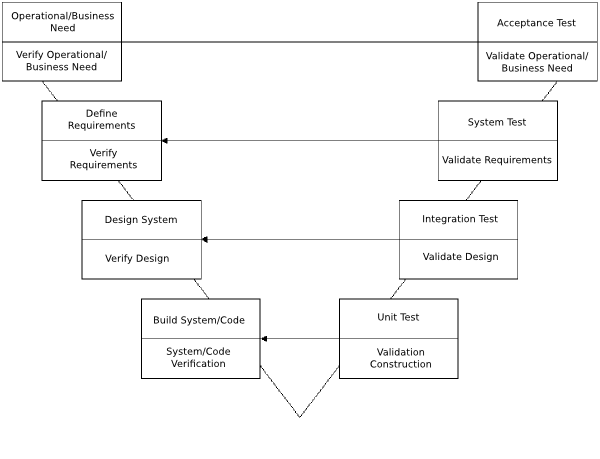
\includegraphics[width=120mm]{img/vmodel.png}
\caption[Schematische Darstellung des V-Modells]{Schematische Darstellung des V-Modells \cite{vmodel}[S. 3]}\label{Abb3}
\end{figure}

Tests können jedoch nicht nur dazu verwendet werden, um Fehler in der Applikation zu finden, sondern auch um einen Überblick über den derzeitigen Stand der Implementation zu gewinnen: Sie geben dem/der EntwicklerIn und ProjektmanagerIn ein direktes Feedback über bereits korrekt implementierte Teile der Software-Spezifikation. Auch Milestones können durch Tests definiert werden. \cite{test_auto}[S. 2]

Zudem ist eine Abschätzung riskanter Bereiche möglich, die durch eine erhöhten Testbedarf bestimmter Bereiche offensichtlich wird. \cite{testing_apps_on_web}[S. 34]


\section{Manuelle Tests}
Manuelle Tests eignen sich vor allem im Bereich des System Tests und Acceptance Tests, da sich diese Bereiche oft schwer komplett automatisch testen lassen. Darunter fallen z.B. Kontrollen der Übersetzungen und der Dokumentation, Usability Tests, externe Beta Tests, Security Tests und explorative Tests. \cite{test_large_systems}[S. 61]


\section{Automatisierte Tests}
Da die vorhandenen Tests durch die Einbindung in den Entwicklungsprozess öfters durchgeführt werden müssen, kann durch das repetetive Durchführen immergleicher Prozesse beim/bei der TesterIn schnell eine gewisse Eintönigkeit und Genervtheit entstehen. Das wiederum kann unter anderem dazu führen, dass TesterInnen im Laufe der Zeit bestimmte Tests nicht korrekt oder ineffizient ausführen. 

Die Lösung des Problems ist die teilweise Automatisierung des Testprozesses. Diese erlaubt bei zukünftigen Testdurchläufen nicht nur eine starke Reduzierung des Zeitaufwandes pro Durchlauf, sondern ermöglicht es auch, die Tests rund um die Uhr durchzuführen. Oft werden am Abend alle zeitintensiven Tests gestartet, damit die EntwicklerInnen am nächsten Morgen einen guten Überblick darüber haben, was nicht oder nicht mehr funktioniert. \cite{test_auto}[S. 22-23]

Es gibt mehrere Faktoren, die bei der Entscheidung der Automatisierung berücksichtigt werden müssen: 

\begin{itemize}
  \item Es muss klar sein, dass der Aufwand der Testerstellung einen wirtschaftlichen Nutzen hat. Bei einer sehr kleinen und unkritischen Applikation kann es sich z.B. nicht lohnen, Tests zu automatisieren. Dies liegt unter anderem daran, dass Tests erst über einen längeren Zeitraum ihre volle Stärke ausspielen. \cite{eval_regression}[S. 12]
  \item Das Personal muss über eine dementsprechende Ausbildung verfügen, die Tests zu automatisieren. \cite{eval_automat_webapp_test}[S. 37]
  \item Es eignet sich nicht jede Testart zur vollkommenen Automatisierung. Währen Unit-Tests und Integration Tests sehr gut automatisiert werden können, ist es schon schwieriger System und Acceptance Tests zu automatisieren. 
\end{itemize}


\section{Grenzen von Software-Tests}
Software-Tests können nie eine komplett fehlerfreie Software garantieren. Es kann höchstens eine Fehlerabwesenheit für jene Fälle garantiert werden, welche mit Tests abgedeckt wurden. \cite{eval_regression}[S. 12]. 

Dies resultiert unter anderem daraus, dass die Anforderungen an die Software oft nicht komplett spezifiziert oder zu ungenau formuliert sind. Zusätzlich steigt die Komplexität der Applikation im Laufe der Entwicklung stark an. Ein weiterer Grund stellt die oft schier unbegrenzten Möglichkeiten an unterschiedlichen Eingaben dar. \cite{software_qual}[S. 243].

Die implementierten Testfälle müssen auch regelmäßig gewartet und aktualisiert werden, um ihre Effektivität zu gewährleisten, denn diese nimmt auf Dauer ab. Es ensteht eine sogenannte \glqq Testresistenz\grqq\cite{eval_regression}[S. 12], die daraus resultiert, dass die bestehenden Tests nur bekannte Fehlerfälle abdecken und keine neuen, mögliche Fehlerfälle berücksichtigen. \cite{eval_regression}[S. 12-13]

\chapter{Testplan}

Mit dem Erstellen des Projektplanes sollte gleichzeitig auch ein Testplan erstellt werden \cite{eval_automat_webapp_test}[S. 24]. Dieser erlaubt, den Testprozess näher zu spezifizieren und somit den erforderlichen Aufwand besser abschätzbar zu machen \cite{test_large_systems}[S. 18]. Sollte es notwendig sein, kann damit der Testprozess auch an ein externes Team ausgelagert werden. Wird der Testplan zudem in den Abnahmenkriterien verankert, reduziert sich das Projektrisiko durch klar definierte Kriterien. \cite{eval_automat_webapp_test}[S. 26]

\section{Inhalt}
Im Testplan werden unter anderem folgende Punkte behandelt \cite{test_auto}[S. 3]:

\begin{itemize}
	\item Was wird getestet? Welche Bereiche besitzen eine höhere Priorität als andere?
	\item Wo wird getestet? Mit welchen Konfigurationen, Soft- und Hardware Plattformen respektive Versionen werden getestet?
	\item Wie wird getestet? mit welchen Tools wird getestet?
	\item Wer testet?
	\item Wie lange wird getestet? Bis wann muss ein Test erfolgreich absolviert werden?
	\item Was wird nicht getestet?
\end{itemize}


\section{Ablauf}
Da die Entwicklung der Applikation meistens unter einem hohen Zeitdruck abläuft\cite{software_qual}[S. 244] und der Testprozess zudem teuer ist \cite{eval_regression}[S. 24], ist es wichtig, Testfälle heraus zu arbeiten, zu priorisieren und effektiv zu verteilen. Auch Endkriterien sollten für die Tests veranschlagt und eine optimale Teststrategie gewählt werden.

Danach folgt die Überprüfung des Testplans. Hier wird überprüft, ob die einzelnen Testfälle genau genug beschrieben worden sind, um daraus die jeweiligen Testfälle erstellen zu können. Auch die Effiktivität der Teststrategien wird überprüft. Diese Prüfung findet nicht nur einmal statt, sondern wiederholt sich mehrfach im Testprozess. Dies hängt damit zusammen, dass die Anforderungen an die Software im Laufe der Implementation immer konkreter werden und somit auch neue, mögliche Fehlerfälle enstehen können.\cite{eval_regression}[S. 25] 

Ist der Testplan soweit fertig, kann ein Zeitplan für die einzelnen Testfälle erstellt werden. In weiterer Folge werden die einzelnen Tests an die TesterInnen vergeben. Diese können nun mit der Erstellung der konkreten Testfälle beginnen können.

Manche Tests haben eine sehr hohe Laufzeit. Um den Ablauf daher zu beschleunigen, wird ein Smoke-Tests erstellt. Der Smoke-Test testet grobe Szenarien der Applikation. Schlagen diese fehl, sind weitere Testdurchläufe nicht notwendig und der Testdurchlauf kann abgebrochen werden. 

Nach dem Ausführen der Tests wird ein Bericht erstellt. Je nach Ausgang der Tests muss der Testplan angepasst werden. Verliefen alle Tests positiv, kann das die jeweilige Phase abgeschlossen werden. \cite{eval_regression}[S. 26]


\section{Vorteile eines Testplans}

Aufgrund der Dokumentation der Testfälle, ergeben sich zusätzlich folgende Vorteile:

\begin{itemize}
	\item Fehlende Testfälle können schnell erkannt werden \cite{test_large_systems}[S. 18]
	\item Redundante Testfälle werden identifziert, Testfälle können zusammegelegt werden um Zeit zu sparen \cite{testing_apps_on_web}[S. 34]
	\item Verschiedene Testbereiche können an mehrere Personen mit unterschiedlichen Fachkenntnissen verteilt werden um Personalengpässe zu vermeiden \cite{test_large_systems}[S. 19]
	\item Ineffiziente Test-Tools und Test-Strategien können erkannt und verbessert werden \cite{eval_regression}[S. 25]
	\item Geschäftskritische Bereiche und solche mit einer erhöhten  Fehleranfälligkeit werden sichtbarer \cite{testing_apps_on_web}[S. 34]. Dies ist vor allem wichtig, da Fehler ungleich verteilt sind und in bestimmten Bereichen häufiger vorkommen als in anderen \cite{eval_regression}[S. 12]
	\item Sinnlose Testfälle und Testbereiche können aussortiert werden 
	\item Abhängigkeiten der Testfälle untereinander und der Implementation werden transparent und erlauben schnell auf Änderungen zu reagieren\cite{test_auto}[S. 4]
\end{itemize}


\chapter{Zusätzliche Herausforderungen beim Testen von Web-Applikationen}
Eine Web-Applikationen unterscheidet sich an mehreren Stellen von einer klassichen Applikation, was das Testen und das Auffinden von Fehlern zusätzlich erschwert. Die Hauptunterschiede sind:

\begin{itemize}
	\item Modularer Aufbau
	\item Plattformunabhängigkeit
	\item Session Modell
\end{itemize}


\section{Modularer Aufbau}

Im Gegensatz zu klassischen Desktop- oder Mobil-Applikationen bestehen Web-Applikationen wegen ihrer Client-Server-Architektur immer aus mehreren Modulen (Abbildung \ref{Abb4}). Diese Module sind meist über ein Netzwerk miteinander verbunden.

Durch diesen modularen Aufbau ist es besonders schwer einen Fehler zu lokalisieren. Ein Fehler kann z.B. durch einen Fehler im Quellcode des Applikations-Servers oder durch ein Netzwerkproblem entstanden sein. \cite{testing_apps_on_web}[Foreword]

\begin{figure}[h!]
\centering
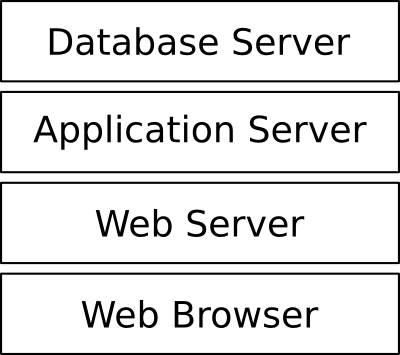
\includegraphics[width=50mm]{img/webstack.png}
\caption[Typischer Aufbau einer Web-Applikation]{Typischer Aufbau einer Web-Applikation}\label{Abb4}
\end{figure}

\section{Unterstützung mehrerer Plattformen}
Web-Applikationen laufen auf einer Vielzahl verschiedener Plattformen, Server- und Clientseitig. Dies ermöglicht dem/der EntwicklerIn Zeit und Aufwand zu sparen, befreit ihn/sie jedoch nicht von der Aufgabe, sicher zu stellen, dass die Applikation auf möglichst vielen Plattformen korrekt ausgeführt wird.

Während auf der Serverseite die jeweilig zu verwendenden Plattformen noch vom/von der BetreiberIn festlegbar sind, sprich welches Betriebssystem und welche Datenbank eingesetzt wird, ist dies auf der Clientseite schon nicht mehr möglich. 

Die BesucherInnen der Webseite verwenden unterschiedliche Web-Browser auf verschiedenen Betriebssystemen in unterschiedlichen Versionen. Auch können unterschiedliche Plugins und Fonts in unterschiedlichen Versionen installiert sein \cite{testing_apps_on_web}[Foreword]. Dies erhöht den Testaufwand, da bestimmte Funktionen nicht vorhanden sein bzw. anders funktionieren können \cite{caniuse}.

Eine weitere Herausforderung von clientseitigem Code stellt die asynchrone und eventbasierte Programmierung dar. Dies erschwehrt nicht nur die Erstellung von Testfällen sondern erhöht auch die möglichen Kombinationen, in der die Events eintreten können. Die Möglichkeit, dass durch eine Aktion, z.B. ein Mausklick auf einen Link, mehrere Events ausgelöst werden können erhöht die Komplexität noch weiter. \cite{testing_apps_on_web}[S. 18]

All diese Probleme werden durch eine zunehmende Verlagerung der Applikations-Logik von der Server- auf die Clientseite\cite{testing_apps_on_web}[S. 13] noch weiter verstärkt. 

\section{Session Modell}
Eine weitere Herausforderung stellt das Session Modell von Web-Applikationen dar: viele Web-Applikationen verwenden nur eine Session pro NutzerIn, erlauben aber mehrere gleichzeitige Logins. Werden mehrere Instanzen der Applikation gestartet - z.B. loggt sich der/die NutzerIn auf dem Mobiltelefon und dem Laptop auf der Webseite ein - kann dies zu Synchronisationsproblemen zwischen den einzelnen Instanzen führen: Wird in einer Instanz ein Eintrag gelöscht, kann dieser durch eine fehlerhafte Synchronisation in einer andere Instanz immer noch existieren und in weiterer Folge zu Fehlern führen. \cite{testing_apps_on_web}[S. 20]


Diese Vielfalt an verschiedenen möglichen Konfigurationen und Herausforderungen erfordert eine neue Herangehensweise an das Thema Software-Test: Die bestehenden Techniken sind \glqq zwar auch notwendig, aber nicht ausreichend, um die Qualität der Applikation sicherzustellen\grqq\ \cite{eval_automat_webapp_test}[S. 18]


\chapter{Projektumfeld}
Die Tests wurden im Rahmen eines Praktikums bei onwCloud Inc. erstellt, um die News Reader App \emph{News} zu testen. Die App setzt auf die ownCloud\cite{owncloud} Plattform auf.

ownCloud ist eine Open Source Web-Applikations-Plattform, welche oft genutzte Cloud Dienste wie z.B. Kalendar, Kontakte, Dateiupload und Synchronisation zur Verfügung stellt. Sie ist in PHP und JavaScript geschrieben, und kann von jedem/jeder NutzerIn auf seinem/ihren privaten Server installiert und verwendet werden. Um Unterschied zu anderen großen Cloud-Service-Anbietern wie Google und Microsoft liegt die Kontrolle der Daten damit beim/bei der NutzerIn. 

\section{Setup auf der Serverseite}
Auf der Serverseite wird PHP in der Version 5.3 eingesetzt. Als Inversion of Control Container kommt Pimple\cite{pimple} zum Einsatz. Als Test-Framwork wird PHPUnit\cite{phpunit} in der Version 3.8 eingesetzt.

Für die Erstellung und Einrichtung der VMs werden Vagrant\cite{vagrant} und Chef\cite{chef} verwendet. Vagrant erlaubt das einfache Erstellen und starten von VMs. Chef erlaubt durch das Verwenden sogenannter \emph{Cookbooks} und \emph{Recipes} eine einfache Installation und Konfiguration von häufig verwendeten Software-Paketen durch Ruby Skripts.

\section{Setup auf der Clientseite}
Die Clientseitige Logik ist mit JavaScript und dem JavaScript Framework AngularJS\cite{angular} in Version 1.0 umgesetzt. AngularJS ist ein MV* Framework und erlaubt eine einfache Trennung der Präsentation und der Logik. Da AngularJS bereits einen Inversion of Control Container mitliefert, wird dieser verwendet. 

Die JavaScript Tests werden mithilfe von Karma\cite{karma}(früher Testacular) 0.8 ausgeführt und basieren auf dem JavaScript Unit Test Framework Jasmine 1.3.1 \cite{jasmine}. 

Die Acceptance und System Tests wurden mit Cucumber 1.3.2 \cite{cucumber} erstellt. Cucumber bietet die Möglichkeit, bereits erstellte User-Stories zu parsen und mit Selenium im Browser auszuführen.


\chapter{Unit Test}
Unit Tests werden verwendet, um Klassen, Module oder einzelne Komponenten zu testen. Sie sind Whitebox Tests, sprich die Implementationsdetails sind bekannt\cite{betrieb}[S. 26], und werden üblicherweise vom ProgrammiererInnen selbst erstellt. 

Da Unit Tests eine Komponente isoliert von anderen Komponenten testet, werden Abhängigkeiten oft mit Mocks (auch Stubs genannt) ersetzt. Dieses Mocks implementieren die Methoden und Attribute, von denen die geteste Komponente abhängt. 

Viele Test-Framworks wie PHPUnit oder Jasmine liefern eigene Mock-Frameworks, mit welchen die Erstellung vereinfacht wird. Ein Mock in PHPUnit sieht in etwa so aus:

\lstinputlisting[language=java]{src/mock.php}

\section{Häufige Probleme}
Das Web ist noch recht jung und entwickelt sich rasant. Wurde es früher nur für Webseiten eingesetzt, sollen nun auf einmal komplette Applikationen entstehen. Dies überfordert viele Entwickler und resultiert oft in halbgaren Architekturen und schlampigen Umsetzungen. 


\subsection{Fehlende Trennung von Logik und Präsentation}
Die mit Abstand am beliebtesten Clientseitige JavaScript Library ist jQuery. Im Jahr 2011 verwendeten laut Alexa 45\% der Top 100.000 Webseiten eine JavaScript Library. Von diesen 45\% entfielen 63\% auf jQuery. \cite{jquery}[S. 107-108]

jQuery ist sehr einfach zu verwenden \cite{jquery}[S. 110], verleitet jedoch den/die ProgrammierIn aufgrund der Funktionsweise dazu, Präsentation und Logik stark miteinander zu verweben. Dies liegt unter anderem daran, dass die meisten jQuery-Methoden einen Selektor als ersten Parameter erwartet. Dieser Selektor funktioniert ähnlich wie ein CSS Selector und selektiert bestimmte Element im DOM. \cite{jquery_selectors}

Folgender Code soll dieses Problem verdeutlichen: Der angeführte Code führt einen AJAX Request aus und gibt abhängig von der zurückgegebenen Datenstruktur einen unterschiedlichen Text aus:

\lstinputlisting[language=Html]{src/jquery.html}
\lstinputlisting[language=JavaScript]{src/jquery.js}

Durch das verwenden des Selektors \emph{\#field .info span} ist der JavaScript Code nun abhänig von der HTML Struktur der Webseite. Verändert ein Designer  die Struktur des HTML-Codes, beispielsweise um die Ausgabe an einen anderen Ort zu verschieben, besteht die Gefahr, dass der Selektor nicht mehr die gewollten Elemente selektiert und damit der JavaScript-Code nicht mehr funktioniert.

Auch Serverseitig kann durch eine Verwebung von Präsentation von Logik schwer zu testender Code entstehen.

\subsection{Verwendung von Globalen Objekten und Variablen}
JavaScript macht es einfach, globale Variablen zu verwenden: Es unterstützt nicht nur implizite \emph{Globals}\cite{js_patterns}[S. 11], sondern regelt den Zugriff auf das DOM über das globale \emph{window} Objekt\cite{js_patterns}[S. 13].

Dadurch werden ProgrammiererInnen dazu verleitet, globale Variablen und Objekte zu benutzen. Das wiederum erschwert die die Testbarkeit, da eine implizite Abhängigkeit ensteht, die für den/die TesterIn nicht sofort offensichtlich ist. Auch wird es schwieriger, den Code in Isolation zu testen.

Jedoch nicht nur JavaScript sondern auch PHP setzt auf globale Variablen: Durch den Einsatz von \emph{Super-Globals} (z.B. \$\_POST oder \$\_SERVER) ist es schwer, eine komplette Isolation von globalen Variablen zu erreichen.

\section{Lösungsansatz}
Die vorher aufgezeigten Probleme können mit Hilfe folgende Techniken gelöst werden:

\begin{itemize}
	\item Trennung der Logik und Präsentation durch Templates
	\item Vermeidung von globalen Objekten und Variablen
	\item Verwendung der Software-Patterns Dependency Injection und Inversion of Control, um Abhängigkeiten von Objekten und Funktionen offensichtlich und konfigurierbar zu machen
\end{itemize}

Um dies zu erreichen wird auf der Clientseite das JavaScript Framework \emph{AngularJS}\cite{angular}, auf der Serverseite der Inversion of Control Container Pimple\cite{pimple} und ownCloud Templates eingesetzt.


\section{Serverseitige Unit Tests}
Durch die Verwendung von Pimple lässt sich nun die Konstruktion der Klassen konfigurieren, indem die Abhängigkeiten im Container definiert werden. Auch Super-Globals können hier injectbar gemacht werden, damit der Code unabhängig von globalen Variablen wird. 

Ein Beispiel für die Container Konfiguration könnte so aussehen:
\lstinputlisting[language=java]{src/pimple.php}

Dazu lassen sich nun einfach Unit Tests erstellen, da die Klasse komplett vom globalen Zustand isoliert wurde. Ein konkreter Unit Test könnte so aussehen:

\lstinputlisting[language=java]{src/phpunit.php}
\lstinputlisting[language=java]{src/phpunittest.php}


\section{Clientseitige Unit Tests}
Auf der Clientseite wird als JavaScript Framework AngularJS eingesetzt. AngularJS erlaubt das Erstellen eigener HTML-Attribute und HTML-Elemente. Diese werden \emph{Directives} genannt und werden für die Darstellungslogik verwendet.

Mit AngularJS würde das vorige jQuery Beispiel in 6.1 in etwa so aussehen:

\lstinputlisting[language=Html]{src/angular.html}
\lstinputlisting[language=JavaScript]{src/angular.js}

Das \emph{Scope} dient als Schnittstelle zwischen der Logik und der Präsentation und erlaubt einen bidirektionalen Datenaustausch. Beide Layer sind nun sauber voneinander getrennt: Der JavaScript Code referenziert keine DOM-Elemente mehr und so kann so isoliert getestet werden. Außerdem ist es nicht mehr möglich, durch bloßes Verschieben des HTML-Codes Fehler in der JavaScript Logik auszulösen.

AngularJS bietet zudem einen Inversion of Control Container um dynamisch Abhängigkeiten unter den Objekten und Funktionen aufzulösen. Häufig benutzte globale Objekte werden schon fertig konfiguriert mitgeliefert: das \emph{window} Objekt etwa kann durch den Service \emph{\$window} injected werden. Dadurch können die Abhängigkeiten einfach in den Tests durch Mocks ausgetauscht werden.

Für das oben aufgeführte Beispiel kann nun ein dazugehöriger Unit Test erstellt werden: Für den AJAX Request wird das \emph{\_\$httpBackend\_} Mock injected. Dies erlaubt den asynchronen Request in einen synchronen umzuwandeln. Auch ein neues Scope wird erstellt, um das korrekte Binding zwischen Präsentation und Logik testen zu können.

\lstinputlisting[language=JavaScript]{src/angularunit.js}

\section{Vor- und Nachteile}

Zu den Vorteilen von Unit Tests zählen:

\begin{itemize}
  \item Gute Paralellisierbarkeit
  \item Sehr schnell ausführbar
  \item Früh einsetzbar
  \item Erlaubt die Aufteilung in kleine Teilprobleme
  \item Zeigt schwer zu verwendende Interfaces auf
\end{itemize}

Viele dieser Vorteile werden durch den Einsatz von Mocks erreicht, die die konkreten Implementationen ersetzen.

Nur Unit Tests alleine reichen jedoch nicht aus, um das Projekt komplett abzudecken, denn Unit Tests\cite{test_large_systems}[S. 52]\cite{betrieb}[S. 28]:

\begin{itemize}
  \item testen keine Kommunikation zwichen den Modulen
  \item testen keine Systemschnittstellen wie z.B. Datenbanken
\end{itemize}

\chapter{Integration Test}
Integration Tests werden verwendet, um die Kommunikation zwischen einzelnen Klassen, Modulen und Komponenten und den Programm-Fluss zu testen. Sie funktionieren ähnlich wie Unit Tests, verwenden jedoch je nach Implementations-Strategie wenig bis keine Mocks und testen weniger Implementationsdetails\cite{test_large_systems}[S. 53-54]. Auf ein Integration Test Quellcode Beispiel wird deshalb verzichtet. 

Durch die vielen möglichen Kombinationen der einzelnen Module gibt es keine allgemein gültige Implementations-Strategie \cite{betrieb}[S. 29]. Die zwei häufigsten verwendeten Methoden zur Erstellung der Testfälle sind:

\begin{itemize}
	\item Nicht Inkrementelle Testfallerstellung
	\item Inkrementelle Testfallerstellung
\end{itemize}

\section{Nicht Inkrementelle Testfallerstellung}
Wird die nicht inkrementelle Testfallerstellung genutzt, werden die nicht vorhandenen Module mit Mocks ersetzt. Diese werden am Schluss dann durch die aktuelle Implementation ausgetauscht.

Dies mag vor allem am Anfang sehr aufwendig erscheinen, erlaubt jedoch schon früh die Kommunikation zwischen den einzelnen Bereichen zu testen. Auf diese Weise kann sehr schnell ein Überblick über den Implementationsstand der Software erlangt werden. Diese Methode eignet sich daher besonders für Agile Software-Entwicklung. \cite{test_large_systems}[S. 54-59] 

Typische Strategien der nicht inkrementellen Testfallerstellung beinhalten\cite{test_large_systems}[S. 54]:

\begin{itemize}
  \item Big-Bang Testing: Möglichst viele fertige Module werden in einen Test integriert
  \item Transaction Testing: Alle Module die zu einer Transaktion gehören werden in einem Test vereint
\end{itemize}


\section{Inkrementelle Testfallerstellung}
Bei der inkrementellen Testfallerstellung werden wenig bis gar keine Mocks erstellt. Stattdessen wird immer versucht, auf den bisherig erstellten Modulen aufzubauen. Dadurch werden die zuerst erstellten Module am Besten getestet.\cite{test_large_systems}[S. 54-59]

Dies eignet sich vor allem dann, wenn es bestimmte Module mit einer hohen Komplexität und Fehlerdichte gibt und das Erstellen von Mocks sehr schwer und aufwendig ist. \cite{test_large_systems}[S. 59]

Typische Vertreter der inkrementellen Testfallerstellung sind\cite{test_large_systems}[S. 54-55]:

\begin{itemize}
  \item Top-Down: Die Module auf dem höchsten Level werden zuerst erstellt
  \item Bottom-Up: Die Module auf dem niedrigsten Level werden zuerst erstellt
  \item Hardest First: Die schwierigsten oder kritischten Module werden zuerst erstellt
  \item Thread Testing: Es wird versucht, einen zusammenhängenden Strang an Funktionen zu erstellen, welcher dann komplett getestet werden kann
  \item Availability Testing: Nur Module, welche schon durch Unit Tests getestet worden sind, werden integriert
\end{itemize}

\section{Vor- und Nachteile}
Integration Tests haben folgende Vorteile:

\begin{itemize}
  \item Testen die Kommunikation und das Zusammenspiel der Komponenten
  \item Testen wichtige Szenarien der einzelnen Module
\end{itemize}

Zu den Nachteilen gehören:

\begin{itemize}
  \item Langsamer als Unit Tests, da ganze Sub-Systeme getestet werden
  \item Kein Test der Systemschnittstellen
\end{itemize}


\chapter{System Test}
System Tests werden verwendet um das Zusammenspiel zwischen dem System und der Applikation zu testen. Sie beinhalten sowohl funktionale (z.B. Installations Tests) als auch nicht funktionale Tests (z.B. Security, Usability oder Performance Tests)\cite{betrieb}[S. 30]. Diese Tests \glqq werden meistens nicht mehr von den Entwicklern selbst durchgeführt, sondern von unabhängigen Tester bzw. Test-Teams.\grqq\cite{eval_regression}[S. 17]

Da die Tests auf einem dem/der Kunden/Kundin ähnlichen System ausgeführt werden, ist es gut, den/die Kunden/Kundin in den Test zu involvieren. Dies gestaltet sich oft als schwierig, da der/die Kunde/Kundin meist nicht die nötige Expertise mitbringt, um die exakten Anforderungen und Testfälle zu erstellen. Als Lösungsmöglichkeit bietet sich hier die Zusammenarbeit mit einem qualifizierten Team des/der Kunden/Kundin \cite{test_large_systems}[S. 60]

\section{Lösungsansatz}
Um die Web-Applikationen sowohl Server- als auch Clientseitig testen zu können, muss eine Entsprechende Möglichkeit bestehen, die verschiedenen System zu simulieren. Dazu werden verschiedenen VMs mit den unterstützten Systemen erstellt. Dann werden die automatisierbaren Tests auf den jeweiligen Systemen ausgeführt, nicht automatisierbare Tests wie etwa die Korrektur der Übersetzungen wird an Test-Teams ausgelagert.

\section{Serverseitige System Tests}
Es ist schwierig, die Tests in Server- und Clientseitige Tests zu spalten, da das ganze System getestet wird. Clientseitige Tests testen somit auch Serverseitige Funktionalitäten. Bestimmte Tests wie Performance Tests müssen z.B. in Kombination durchgeführt werden.

Die Serverseitigen Tests reduzieren sich deshalb auf das Erstellen und Einrichten der jeweiligen VMs für den Serverseitigen Code und auf das Testen von\cite{test_large_systems}[S. 60-66]:

\begin{itemize}
  \item Security: Statische Code Analysen können mit Tools durchgeführt werden
  \item Konfiguration: Mit einem Skript werden verschiedene Konfigurationen erstellt und getestet
  \item Kompatibiltät der Applikation mit dem Server Betriebssystem und den serverseitigen Applikationen: Wird mit Chef und Vagrant durchgeführt
  \item Recovery Funktionen: Falls verfügbar mittels Skript gestartet
  \item Performance und Speicherverbrauch: Mit einem Skript werden verschiedene, gleichzeitige Anfragen an den Server erstellt, der Arbeitsspeicher wird auf das spezifizierte Minimum reduziert
  \item Installation: Wird durch den Clientseitigen Installationsdialog Server- und Clientseitig getestet
  \item Zuverlässigkeit: Kommt darauf an, ob die Anforderungen testbar formuliert sind, z.B. mit durchschnittlicher Fehlerrate pro Stunde
\end{itemize}

\section{Clientseitige System Tests}
Die Clientseitigen System Tests werden auf unterschiedlichen Web-Browsern ausgeführt. Auch zusätzliche VMs für Windows und Mac OS X sind notwendig um verschiedene Versionen des Internet Explorers respektive Safari zu testen. Die restlichen Tests können unter Linux VMs durchgeführt werden.

\subsection{JavaScript Tests}
Der JavaScript Testrunner Karma erlaubt die Konfiguration verschiedener Web-Browser unter welchen die JavaScript Unit Tests ausgeführt werden können. Dadurch kann sichergestellt werden, dass der JavaScript Code auf allen Systemen wie gewünscht funktioniert.

\subsection{User-Interface Tests}
Für die User-Interface Tests wird Cucumber verwendet. Die gewünschten User-Stories werden in Gherkin (der User-Story Grammatik) spezifiziert. Danach lassen sich die Methoden erstellen, die die User-Stories parsen und in den verschiedenen Browsern durchführen.

Folgendes Beispiel loggt sich ein und überprüft, ob bei einem Klick auf einen Button das entsprechende Formular sichtbar wird:

\lstinputlisting{src/create.feature}

Die User-Story lässt sich nun mit folgenden Schritten parsen und testen:

\lstinputlisting[language=ruby]{src/create_steps.rb}

\section{Vor- und Nachteile}
Durch die Simulation der verschiedenen Umgebungen ergeben sich folgende Vorteile \cite{test_large_systems}[S. 60-66]:

\begin{itemize}
  \item Sicherheit, dass die Applikation auf unterschiedlichen Plattformen funktionert
  \item Auch nicht funktionale, aber manchmal projektkritische Anforderungen wie Performance testbar
\end{itemize}

Da für die verschiedenen Plattformen jeweils Testumgebungen gestartet werden müssen, entstehen dadurch vor allem folgende Nachteile:

\begin{itemize}
  \item Lange Startzeit der Testumgebungen
  \item Lange Laufzeit der Tests
  \item Dadurch langsame Entwicklung der Tests
  \item Fehler durch großen Bereich schwer lokalisierbar
  \item Sehr schwierig die exakte Testumgebung zu reproduzieren
  \item Schwer automatisierbar vor allem bei nicht funktionalen Tests wie Usability Tests
\end{itemize}


\chapter{Acceptance Test}
Beim Acceptance Test wird die Applikation auf die Anforderungen des/der Kunden/Kundin geprüft \cite{test_large_systems}[S. 66]. Der Test ist erforderlich, um eine erfolgreiche Abnahme durch den/die Kunden/Kundin zu erreichen. Da es vor allem im Interesse des/der Kunden/Kundin ist, eine wie im Vertrag vereinbarte funktionierende Software zu erhalten, ist er/sie meistens der HaupttesterIn.

Zu den verschiedenen Tests zählen \cite{betrieb}[S. 33-34]:

\begin{itemize}
   \item \glqq Test auf verträgliche Akzeptanz\grqq
   \item \glqq Test der Benutzbarkeit\grqq
   \item \glqq Akzeptanz durch den Systembetreiber\grqq
   \item \glqq Feldrest (Alpha- und Betatest)\grqq
 \end{itemize} 

Um das Risiko einer verweigerten Abnahme im späten Stadium zu vermindern, können die Acceptance Tests bereits während der Entwicklung mit dem/der Kunden/Kundin zusammen durchgeführt werden, was sich vor allem in einem agilen Software-Projekt anbietet. \cite{eval_regression}[S. 17]

\section{Lösungsansatz}
Dadurch, dass der/die Kunde/Kundin in diesem Fall der/die HaupttesterIn der Software ist, gestaltet es sich schwierig, diesen Prozess zu automatisieren. Es empfiehlt sich, regelmäßige Meetings mit dem/der Kunden/Kundin abzuhalten, damit das Projekt früh genug an die aufkommenden Probleme angepasst werden kann. Außerdem bietet es sich an, die in den während des System Tests erstellten User-Stories integriert werden. Wurden diese vom oder mit Hilfe des/der Kunden/Kundin erstellt, kann der/die HerstellerIn damit argumentieren, dass die verlangten Features komplett umgesetzt wurden.


\chapter{Zusammenfassung}


% TODO: Vergleich zu klassischen apps nochmal erläutern, vor + nachteile vllt auch tabellarisch, abkürzungsverzeichnis weglassen bei nur 2 abkürzungen, mehr abbildungen


%\\[2\baselineskip]
%Hier wird auf Abbildung~\ref{Abb1} verwiesen. 
%\begin{figure}[htbp]
%\centering
%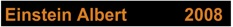
\includegraphics[width=75mm]{Buchruecken}
%\caption[Beschriftung eines Buchrückens.]{Beispiel für die Beschriftung eines
%Buchrückens.}\label{Abb1}
%\end{figure}
%%Tabelle~\ref{Tab1} ist ein Beispiel dafür, wie eine Tabelle aussehen könnte.
%\begin{table}[htbp]
%\centering
%\begin{tabular}{ | c | c | c | }\hline
%{\bf Datum} & {\bf Thema} & {\bf Raum}\\ \hline
%\hline
%20. 08. 2008 & Graphentheorie & HS 3.13\\ \hline
%01. 10. 2008 & Biomathematik & HS 1.05\\ \hline
%\end{tabular}
%\caption[Semesterplan "`Angewandte Mathematik"'.]{Beispiel für einen
%Semesterplan "`Angewandte Mathematik"'.}\label{Tab1}
%\end{table}

%\noindent
%Nun ein Beispiel für eine abgesetzte Formel:
%\begin{equation}
%x =  - \frac{p}{2} \pm \sqrt{\left(\frac{p}{2}\right)^2 - q}.
%\end{equation}
%Und eine mehrzeilige Formel:
%\begin{eqnarray}
%f(t)&=& t^2 \label{For1},\\
%g(t) &=& t-1.
%\end{eqnarray}
%Hier wird auf die Formel (\ref{For1}) verwiesen. \\

%\noindent
%So kann zum Beispiel ein \glqq Source-Code\grqq\  angegeben werden: 
%\begin{verbatim}
%for (i=1; i < 10; i++) {...} 
%\end{verbatim}

%\noindent
%Hier ist ein Hyperlink auf die  \href{http://www.technikum-wien.at}{Homepage}
%der FH Technikum Wien. Email-Adressen können so verlinkt werden:
%\href{mailto:homer.simpson@springfield.com}{\texttt{
%homer.simpson@springfield.com}}\\

%\noindent
%In der Bibliothek der Fachhochschule Technikum Wien gibt es verschiedene
%einführende Bücher zum Thema \glqq \LaTeX \grqq, zum Beispiel \cite{kop05},
%\cite{wil06} oder \cite{mgb+05d} (deutsche Version) bzw. \cite{mgb+04e}
%(englische Version). Empfehlenswerte Skripten für \LaTeX-Einsteiger sind z.B.
%\cite{mj00} und \cite{mj95}. Sie sind frei im Internet verfügbar.



% Literaturverzeichnis
% Das Literaturverzeichnis kann auch nach einem allfälligen Anhang positiioniert werden (siehe "`Leitfaden für Bachelor- und Diplomarbeiten"', Version 2.0, Abschnitt 2.9).

% Möglichkeit 1: Erzeugung des Literaturverzeichnisses mit BibTeX:
% Die Quellen sind in der Datei *.bib (hier Literatur.bib) einzugeben. Danach muss diese Vorlage einmal geTeXt werden, dann BibTeX angewendet werden und 
% anschliessend nochmals zweimal geTeXt werden.
% Im Text erfolgt die Zitierung mit dem Anker-Schlüsselwort, z.B. \cite{kop05}.
\bibliographystyle{IEEEtran}
\bibliography{Literatur}

% Möglichkeit 2: Erzeugung eines Literaturverzeichnisses ohne BibTeX:
%\begin{thebibliography}{99}
%\bibitem[kop05]{kop05}
%H.~Kopka, {\em LaTeX, Band 1: Einführung}, Pearson Studium, München, 3.~Auflage, 2005.
%\bibitem[knu98]{knu98}
%F.~Mittelbach, M.~Goossens, J.~Braams, D.~Carlisle, and Ch. Rowley, {\em The LaTeX Companion}, 
%Addison-Wesley, 2nd edition, 2004.
%\end{thebibliography}

% Abbildungsverzeichnis
\listoffigures
\addcontentsline{toc}{chapter}{Abbildungsverzeichnis} % fügt den Eintrag äbbildungsverzeichnis" im Inhaltsverzeichnis hinzu
\newpage

% Tabellenverzeichnis
%\listoftables 
%\addcontentsline{toc}{chapter}{Tabellenverzeichnis} % fügt den Eintrag
%"Tabellenverzeichnis" im Inhaltsverzeichnis hinzu
%\newpage

% Abkürzungsverzeichnis
% Bei Verwendung der Dokumentklasse "scrartcl" ist der Befehlt \addchap{Abkürzungsverzeichnis} durch 
% \addsec{Abkürzungsverzeichnis} zu ersetzen
\addchap{Abkürzungsverzeichnis}
\hspace{-17mm}\begin{tabular}{>{\raggedleft}p{0.2\linewidth} p{0.75\linewidth} p{0.1\linewidth}}

www & World Wide Web\\
CSS & Cascading Style Sheets\\
AJAX & Asynchron JavaScript And XML\\
HTML & HyperText Markup Language\\
DOM & Document Object Model\\
W3C & World Wide Web Consortium\\
MV* & Model View - View Model\\

\end{tabular}

% Anhänge
%\begin{appendix}
%\chapter[Erster Anhang]{überschrift des ersten Anhangs}

%Text Text Text Text Text Text Text Text Text Text Text Text Text Text Text Text
%\end{appendix}

\end{document}
